\documentclass{report}

%preaumbulum
\usepackage[T1]{fontenc}
\usepackage[utf8]{inputenc}
\usepackage[magyar]{babel}

\usepackage{amsmath}
\usepackage{amssymb}

\usepackage{graphicx}
\usepackage{caption}
\usepackage{multicol}
\usepackage{hyperref}
\usepackage{url}


\title{laTEX Beadandó}
\author{Jandzsó György}
\date{\today}

\begin{document}
	\maketitle
	
	\tableofcontents
	\listoffigures
	\listoftables


	\chapter{IoT biztonsági szempontból}
		Az Internet of Things, vagyis az IoT, a mindennapi életünk szerves részévé vált. Az okos otthonoktól a gyártási folyamatokig, az IoT eszközök hatalmas lehetőségeket nyitnak meg számunkra. Azonban ahogy ezek az eszközök egyre inkább beépülnek a mindennapjainkba, a biztonságuk kulcsfontosságúvá válik. A korlátozott erőforrások, a gyenge jelszavak és hitelesítési módszerek, valamint az érzékeny adatok kezelése mind olyan kihívások, amelyekkel szembe kell néznünk. 

		\section{Generált leírás}
			Az IoT (Internet of Things) eszközök gyors terjedése és széles körű alkalmazása új kihívásokat jelent a biztonság területén. Az IoT eszközöknek rendszerint korlátozott erőforrásaik vannak, amelyek miatt gyakran nem lehet rajtuk olyan erős biztonsági mechanizmusokat implementálni, mint az asztali vagy mobil eszközökön. Ennek eredményeként az IoT eszközök gyakran sebezhetővé válnak a kiberbűnözők és más támadók számára.
			Az egyik legfontosabb kérdés az IoT eszközök biztonságával kapcsolatban az alapértelmezett jelszavak és hitelesítési módszerek használata. Sok esetben az IoT eszközök gyártói által előre beállított jelszavakat nem változtatják meg a felhasználók, vagy olyan egyszerű jelszavakat használnak, amelyek könnyen kitalálhatók. Ez lehetővé teszi a támadók számára, hogy könnyen hozzáférjenek az eszközhöz és akár irányításuk alá is vehessék azt.
			A másik fontos szempont az adatvédelem és adatbiztonság. Az IoT eszközök gyakran érzékeny adatokat gyűjtenek és továbbítanak, például a felhasználók személyes adatait vagy az otthonok biztonságával kapcsolatos információkat. Az ilyen adatok védelme kritikus fontosságú, hogy megakadályozzuk az illetéktelen hozzáférést és a bizalmas információk kiszivárgását.
			Az IoT biztonságának javítása érdekében számos lépésre van szükség. Elengedhetetlen, hogy az IoT eszközöket szigorú biztonsági irányelvek és protokollok szerint tervezzék és fejlesszék. Emellett fontos, hogy a felhasználók számára egyszerű és hatékony módon biztosítsák az eszközök beállításait és frissítéseit, hogy minimalizálják a sebezhetőségeket és javítsák a biztonságot.
			Az IoT eszközök biztonsága nemcsak a gyártók és fejlesztők, hanem a felhasználók és az IoT ökoszisztéma más résztvevői számára is közös felelősség. Az együttműködés és a szoros együttműködés révén lehetőség van a fenyegetések felismerésére és kezelésére, így biztonságosabb IoT környezetet teremthetünk mindannyiunk számára.
			
		\section{Összefoglaló a témáról}
			Az IoT eszközök új problémákat vetnek fel, mivel a korlátozott erőforrásaik gyakran nem teszik lehetővé a komoly biztonsági megoldásokat.\footnote{Komolyabb tűzfal és dns-szűrő használatával javítható a probléma}  Ezért igen népszerű célpontok lehetnek a kiberbűnözők szemében. A gyenge jelszavak\footnote{Soha: password123} és hitelesítési módszerek csak rontanak a helyzeten.
			Gyakran gyűjtenek érzékeny személyes adatokat, így az adatbiztonság fontossága jelentős. Szigorúbb biztonsági irányelvek szerinti tervezésre és fejlesztésre van szükség, valamint a felhasználók számára egyszerű, de biztonságos eszközbeállításokra és rendszeres frissítésekre.
			A biztonság közös felelősség, amelyre a gyártók, fejlesztők és felhasználók együtt kell, hogy törekedjenek.
			Jó és kényelmes dolog az IoT, de jelentős biztonsági kockázattal jár, tehát érdemes figyelni ezekre.





	\chapter{Tételek}
		\section{Ismertesse a verziókezelők fajtáit, nevezzen meg verziókezelő programokat!}
			\subsection{Verziókezelők fajtái és programok}
				A verziókezelők két fő típusa a központi és az elosztott. A központi verziókezelők, mint például a Subversion (SVN) és a Concurrent Versions System (CVS), egy központi szerveren tárolják a fájlok verzióit. Az elosztott verziókezelők, mint például a Git, a Mercurial és a Bazaar, minden fejlesztőnél tárolnak egy teljes másolatot a projekt történetéről.
			
			\subsection{Központi vs Elosztott Verziókezelés}
				A központi verziókezelésnél minden változtatás egy központi szerveren kerül tárolásra. Ez egyszerűsíti a változások nyomon követését, de fennáll a veszélye, hogy ha a központi szerver meghibásodik, akkor a projekt teljes története elveszhet. Az elosztott verziókezelésnél minden fejlesztő rendelkezik a projekt teljes történetének egy másolatával. Ez biztonságosabb, mert ha egy szerver meghibásodik, a projekt története nem vész el.
			
				\begin{table}[htbp]
					    \centering
					    \begin{tabular}{|c|c|c|}
					    \hline
					    \textbf{Központi} & \textbf{Elosztott}  \\
					    \hline
					    SVN & Git \\
					    CVS & Mercurial \\
					    \hline
					    \end{tabular}
					    \caption{Verziókezelők}
					    \label{tab:Verziókezelők}
				\end{table}



			\subsection{Git Fogalmak}
				\begin{description}
					\item [Branch]: Egy önálló fejlesztési ág, amely lehetővé teszi a fejlesztők számára, hogy külön-külön dolgozzanak ugyanazon a projekten.
					\item [Tag]: Egy jelölés egy adott commitra, gyakran használják verziószámok jelölésére.
					\item [Commit]: Egy változás halmaza, amelyet a fejlesztő hozzáad a projekt történetéhez.
					\item [Merge]: Két branch összevonása, ahol a Git automatikusan összefésüli a változásokat, ha lehetséges.
					\item [Rebase]: Egy branch frissítése a legújabb változásokkal egy másik branchről, úgy, hogy a branch történetét újraírja.
					\item [Fetch]: A távoli repository változásainak letöltése a helyi repositoryba, anélkül, hogy összefésülné őket a helyi branchekkel.
				\end{description}
			
			\subsection{Git Flow}
				A Git Flow egy workflow modell, amelyet Vincent Driessen fejlesztett ki, és amely előírja, hogyan kell használni a Gitet a projekt fejlesztésében. A Git Flowban vannak állandó branchek (master és develop), és ideiglenes branchek (feature, release és hotfix branchek).
			
			\subsection{Tesztelés és Life-Cycle Folyamatok}
				A forráskód tesztelése elengedhetetlen a minőségi szoftverfejlesztésben. A tesztelési folyamatok közé tartozik az egységtesztelés, az integrációs tesztelés, a rendszertesztelés és az elfogadási tesztelés. A life-cycle folyamatok kezelése a forráskódra vonatkozóan magában foglalja a verziókezelést, a build automatizálást, a folyamatos integrációt és a folyamatos szállítást/deploymentet. Ezek a folyamatok segítenek a fejlesztőknek a kód minőségének fenntartásában, a hibák korai felismerésében és a gyorsabb szoftverkiszállításban.
		
		\section{Ismertesse a webszolgáltatások típusait, melyiknek mi a formátuma, lényege, eszköze}
			\subsection{Webszolgáltatások típusai}
				
				\section*{SOAP (Simple Object Access Protocol)}
					\textbf{Formátum}: XML alapú üzenetek.\\
					\textbf{Lényege}: Előre meghatározott üzenetformátumokkal működő protokoll, amelyet általában XML-ben kódolnak. \\
					\textbf{Eszközök}: SOAP üzeneteket generáló és fogadó eszközök, mint például SOAP UI.
				
				\section*{REST (Representational State Transfer)}
					\textbf{Formátum}: Általában JSON vagy XML alapú adatátvitel.\\
					\textbf{Lényege}: A HTTP protokollra épülő könnyű, egyszerű és skálázható webszolgáltatásokat definiáló architektúra. \\
					\textbf{Eszközök}: Szinte minden modern programozási nyelv támogatja a REST API-k készítését és hívását.
				
			\subsection{Publikus webszolgáltatások}
				\begin{itemize}
				    \item Google Maps API
				    \item Twitter API
				    \item OpenWeatherMap API
				    \item GitHub API
				\end{itemize}
			
			\subsection{Szolgáltatorientált architektúra (SOA)}
				\section*{Ábra}
					\begin{figure}[h]
					    \centering
					    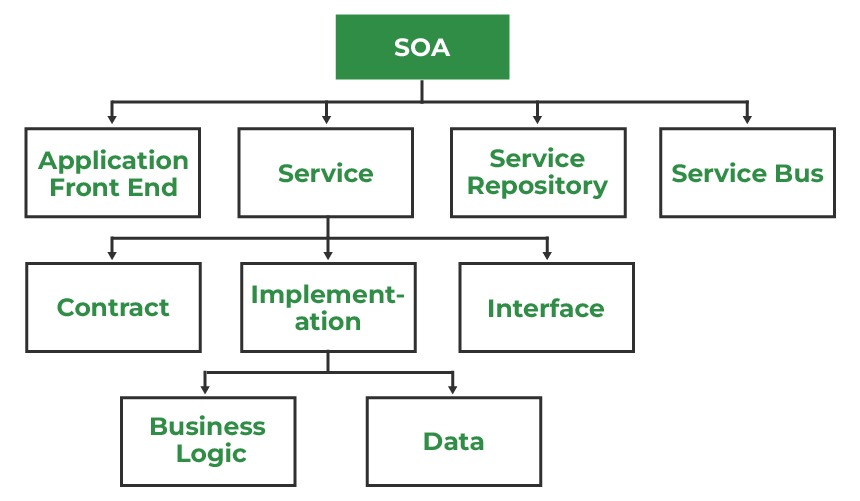
\includegraphics[width=1\textwidth]{figures/SOA.png}
					    \caption{SOA Architektúra}
					    \label{fig:SOA Architektúra}
					\end{figure}
				
				\section*{Lényege}
				A SOA egy olyan szoftverarchitektúra, amelyben a különböző alkalmazások különálló szolgáltatásokként vannak megvalósítva\footnote{Hasonlóan a mikroszolgáltatásokhoz}, amelyeket más alkalmazások fogyasztanak.

				
				\section*{Elvek}
					\begin{enumerate}
					    \item Szolgáltatások újrafelhasználhatósága
					    \item Kompozíció (a szolgáltatások összekapcsolhatósága)
					    \item Láthatóság (a szolgáltatások nyilvánosan elérhetők és dokumentáltak)
					    \item Függetlenség (a szolgáltatások különállóan változtathatók)
					\end{enumerate}
				
			\subsection{REST vs. RPC}
				
				\section*{REST (Representational State Transfer)}
					\begin{itemize}
					    \item Az erőforrásokra épül.
					    \item Állapotmentes kérések.
					    \item HTTP metódusokat (GET, POST, PUT, DELETE) használ az erőforrások manipulálására.
					    \item Például: HTTP GET kérések egy adott erőforrás lekérdezésére.
					\end{itemize}
				
				\section*{RPC (Remote Procedure Call)}
					\begin{itemize}
					    \item Függvényhívásokra épül.
					    \item Állapotfüggő.
					    \item Távoli szolgáltatások hívása speciális RPC protokollokkal.
					    \item Például: A kliens hívja a távoli függvényeket, mint egy lokális függvényt.
					\end{itemize}




		\section{Nem ide illő matematikai probléma}
			Mivel keresve sem találtam matematikai példát a szoftverfejlesztési tételekben, így rögtönöztem:
			\begin{align}
			    f(x) &= x^2 + 2x + 1 = (x + 1)^2
			\end{align}
			
		
			Szintén, a másik kötelező csomag szimbólumai:
			\begin{description}
				    \item Komplex számok: $\mathbb{C}$
				    \item Valós számok: $\mathbb{R}$
				    \item Egész számok: $\mathbb{Z}$
				    \item Természetes számok: $\mathbb{N}$
				    \item Racionális számok: $\mathbb{Q}$
				    \item Tömör halmaz: $\emptyset$
				    \item Egyenlő: $\equiv$
				    \item Nem egyenlő: $\neq$
				    \item Végtelen: $\infty$

			\end{description}
			



		
	\chapter{Nappali képzés}
		A nappali képzés egy intenzív, de megfelelő előnyökkel járó tapasztalat. 
		Lehetővé teszi az anyag megértése során felmerülő kérdések megválaszolását, továbbá a személyes kapcsolatokat a tanárokkal és a szaktársakkal javítja.
		A napod nagyrészt a tanulás köré épül, így nagy elkötelezettséget igényel, dolgozni mellette hétközben, problémás. 
		Fontos, hogy időt és energiát fektess a tanulásba, sőt sajnos az kell legyen a prioritás is.


		\begin{multicols}{2}

			\section{Előnyök}
				 \begin{itemize} 
					\item \textbf{Személyes interakció}: Lehetőség a tanárok és diákok közötti személyes interakcióra.
					\item \textbf{Szociális kapcsolatok}: Új embereket megismerése és a szociális hálózat bővítése.
					\item \textbf{Időbeosztás}: Szigorúbb időbeosztással jár, ami segíthet abban, hogy ne legyen halogatva a feladat.

				\end{itemize}
			\columnbreak
			\section{Hátrányok}
				 \begin{itemize} 
					\item \textbf{Időigényes}: Sokkal több idő ráfordításával jár, mint egy esti vagy levelező szak.
					\item \textbf{Költséges}: Ha helyszín messze van, akkor számolni kell az utazás vagy lakhatás költségével.
					\item \textbf{Nincs rugalmas időbeosztás}:  Kevésbé rugalmas, ami problémás más tevékenységek mellett, mint a munkavégzés.
				\end{itemize}
		\end{multicols}

		

		
	\chapter*{Irodalomjegyzék}
		\begin{thebibliography}{9}
		    \bibitem{ChatGPT} OpenAI (chatGPT), \url{https://openai.com} (\today)
		    \bibitem{SOA} Software Testing – SOA Testing, \url{https://www.geeksforgeeks.org/software-testing-soa-testing/} (\today)
		    \bibitem{Módszertanok} Fejlesztési modellek és módszertanok, \url{https://szit.hu/doku.php?id=oktatas:programozas:fejlesztesi_modellek_es_modszertanok} (\today)
		    \bibitem{Verziókezelő} Verziókezelő rendszer, \url{https://bitbucket.org/product/hu/version-control-software} (\today)
		\end{thebibliography}

\end{document}
